\documentclass[legalpaper, 12pt]{exam}
\usepackage[margin=0.3in]{geometry}
\usepackage[utf8]{inputenc}
% \usepackage{graphics}
\usepackage{color}
\usepackage{amssymb}
\usepackage{amsmath}
\usepackage{enumitem}
\usepackage{xcolor}
\usepackage{cancel}
\usepackage{ragged2e}
\usepackage{graphicx}
\usepackage{multicol}
\usepackage{color}
\usepackage{tikz}
\usepackage{caption}
\usepackage{pgfplots}
\usepackage{physics}
% \pgfplotsset{compat = newest}
\def\F(#1){((#1)^3- 3*(#1))^2}%
\usetikzlibrary{arrows,snakes,backgrounds,patterns,shapes.geometric,calc}

\everymath={\displaystyle}
\renewcommand*{\choicelabel}{(\thechoice)}
\renewcommand*{\choicelabel}{
  \ifnum\value{choice}>1
    \makebox[4em][r]{(\thechoice)}
  \else
    (\thechoice)
  \fi
}

\setlength{\multicolsep}{0.6em}
\printanswers

\renewcommand{\solutiontitle}{\noindent\textbf{Solución: }}
\newcommand{\cancelroot}[1]{%
  \sbox0{$\displaystyle\sqrt{\vphantom{#1}}$}%
  \cancel{\phantom{\usebox0}\hspace{0.5em}}\hspace{\dimexpr-\wd0-0.5em}%
  \sqrt{#1}%
}

\pgfplotsset{compat=1.10}
\usepgfplotslibrary{fillbetween}
\usetikzlibrary{patterns}

\begin{document}
\begin{figure}[t]

\includegraphics[width=0.1\textwidth,height=0.2\textheight,keepaspectratio]{ENCB.png}\hfill

\includegraphics[width=0.14\textwidth,height=0.2\textheight,keepaspectratio]{IPN.pdf}
\end{figure}

\begin{center}
{\vspace*{-3.5cm}\LARGE\textbf{INSTITUTO POLITÉCNICO NACIONAL}} \\\vspace*{0.3cm}
{\Large Escuela Nacional de Ciencias Biológicas -- ENCB}\\\vspace*{0.3cm}
{\huge C\ Á\ L\ C\ U\ L\ O}\\\vspace*{0.3cm}
Tercera evaluación (9/07/2020)

\end{center}
\extraheadheight{-0.5in}
\runningheadrule \extraheadheight{0.1in}
\vspace{0.15in}
\runningheadrule \extraheadheight{0.44in}
% \lhead{\ifcontinuation{Pregunta \ContinuedQuestion\ continua\ldots}{}}
\runningheader{Cálculo Integral }{Tercera Evaluación}{Julio 2020}
\runningfooter{ENCB}
              {\thepage\ of \numpages}
              {}
% \vspace{-0.2in}

\begin{questions}
%%%%%%%%%%%%%%%%%%%%%%%%%%%%%%%%%%%%%
%           QUESTION                %
%%%%%%%%%%%%%%%%%%%%%%%%%%%%%%%%%%%%%
\question  Un derrame de petróleo adopta una forma circular y tiene espesor constante de $\dfrac{1}{50} ft$. Si el petróleo se esta escapando a razón de $40 ft^3/min$. ¿A qué razón está aumentando  el radio de la mancha de petróleo cuando el radio es de $50ft$?
%%%%%%%%%%%%%%%%%%%%%%%%%%%%%%%%%%%%%%
%             ANSWER                 %
%%%%%%%%%%%%%%%%%%%%%%%%%%%%%%%%%%%%%%
\begin{solution}[.2in]
Primero que nada hacemos un dibujo del problema. En este caso se dibuja un cilindro recto circular con altura o espesor constante $h=\dfrac{1}{50}$ y radio $r$ que es el que irá cambiando para $t\geq 0$.\\

\begin{multicols}{2}
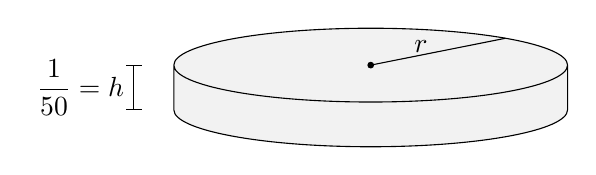
\begin{tikzpicture}[scale=1]
\node [draw, cylinder, cylinder uses custom fill, cylinder body fill=lightgray!20,
cylinder end fill=lightgray!20, shape aspect=4, rotate=90, minimum width=5cm] (c) at
(0,1.8){};

\coordinate(dhtop) at ($(c.before top)!-1*.1!(c.after top)$);
\coordinate(dhbot) at ($(c.after bottom)!-1*.1!(c.before bottom)$);
\coordinate(dhlabel) at ($(dhtop)!.5!(dhbot)$);
\draw[|-|] (dhbot)--(dhtop);
\path (dhlabel) node[left] {$\dfrac{1}{50} = h$};

\coordinate (center) at ($(c.before top)!0.5!(c.after top)$);
\filldraw (center) circle (1pt);
\coordinate (rlabel) at ($(center) !0.5!(c.after top)$);
\coordinate (rtop) at ($(center)!-1*.1!(c.after top)$);

\coordinate (rend) at ($(c.mid east)!0.5!(c.after top)$);
\draw[-, shorten >=-15] (center) -- (rend);
\path (rend) node[outer sep = 10pt, left] {$r$};
\end{tikzpicture}\\
entonces,definimos el volumen de un cilindro rectangular como $V = \pi r^2 h$, sustituyendo $h = \dfrac{1}{50}$ se tiene $V = \dfrac{\pi}{50}r^2$.
\end{multicols}
La razón de cambio del volumen con respecto al tiempo es:
\begin{align}
\dfrac{dV(t)}{dt} = \dfrac{2\pi}{50}r(t)\cdot\dfrac{dr(t)}{dt},\label{uno}
\end{align}
por otro lado, sabemos que el petróleo se esta escapando a razón de $40 ft^3/min$, eso quiere decir que $\dfrac{dV(t)}{dt}=40$, así mismo nos están preguntando la razón de cambio del radio de la mancha de petróleo, por lo que necesitamos encontrar $\dfrac{dr(t)}{dt}$ cuando $r = 50 ft$, entonces de \eqref{uno} se tiene:
\begin{align*}
40 = \dfrac{2\pi}{\cancel{50}}\left(\cancel{50}\right)\cdot\dfrac{dr(t)}{dt},
\end{align*}
por lo tanto la solución es que el radio esta cambiando a razón de $\dfrac{dr(t)}{dt} = \dfrac{20}{\pi}\ ft/min$.
\end{solution}

 \vspace{0.15in}
%%%%%%%%%%%%%%%%%%%%%%%%%%%%%%%%%%%%%
%           QUESTION                %
%%%%%%%%%%%%%%%%%%%%%%%%%%%%%%%%%%%%%
\question Se requiere inscribir un rectángulo dentro de un semicírculo de radio 2. ¿Cuál es el área más grande que puede tener el rectángulo y cuales son sus dimensiones?
%%%%%%%%%%%%%%%%%%%%%%%%%%%%%%%%%%%%%%
%             ANSWER                 %
%%%%%%%%%%%%%%%%%%%%%%%%%%%%%%%%%%%%%%
\begin{solution}
Nuevamente primero hacemos un dibujo del problema
\begin{multicols}{2}
\begin{center}
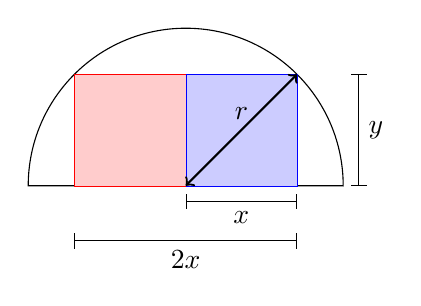
\begin{tikzpicture}
  % Define coordinates
  \def\Radius{2}
  \path
    (-\Radius, 0) coordinate (A)
    -- coordinate (M)
    (\Radius, 0) coordinate (B)
    (M) +(60:\Radius) coordinate (C)
    +(120:\Radius) coordinate (D)
  ;
  % Draw semicircle
  \draw
    (B) arc(0:180:\Radius) -- cycle;
  \filldraw[red, fill=red!20, ultra thin] (-1.41421356,0) rectangle (0,1.41421356);
  \filldraw[blue, fill=blue!20, ultra thin] (0,0) rectangle (1.41421356,1.41421356);
  \draw[|-|](0,-0.2)--node[below]{$x$}(1.41421356,-0.2);
  \draw[|-|](-1.41421356,-0.7)--node[below]{$2x$}(1.41421356,-0.7);
  \draw[|-|](2.2,0)--node[right]{$y$}(2.2,1.41421356);
  \draw[<->,thick](0,0)--node[above]{$r$}(1.41421356,1.41421356);
\end{tikzpicture}
\end{center}
Por lo tanto las medidas del rectángulo que nos interesan serán $ancho = 2x$ y $alto = y$. Dividimos el rectángulo en dos por la mitad, lo que nos quedaría un rectángulo de $ancho = x$ y $alto = y$, denotando con $r$ al radio del semicírculo, por lo tanto tomando uno de los rectángulos pequeños.
\begin{center}
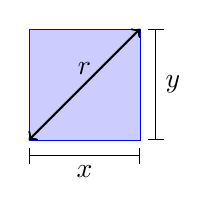
\begin{tikzpicture}[baseline=(current bounding box.north)]
  % Define coordinates
  \filldraw[blue, fill=blue!20, ultra thin] (0,0) rectangle (1.41421356,1.41421356);
  \draw[|-|](0,-0.2)--node[below]{$x$}(1.41421356,-0.2);
  \draw[|-|](1.41421356+0.2,0)--node[right]{$y$}(1.41421356+0.2,1.41421356);
  \draw[<->,thick](0,0)--node[above]{$r$}(1.41421356,1.41421356);
\end{tikzpicture}
\end{center}
por el teorema de Pitágoras decimos que
\begin{align*}
r^2 = x^2 + y^2
\end{align*}
y por lo tanto
\begin{align*}
y = \sqrt{r^2 - x^2}
\end{align*}
entonces el área del rectángulo es
\begin{align}
A(x) = x\sqrt{r^2 - x^2},\label{dos}
\end{align}
cuyo dominio es $D_A = (0,r]$.\vspace*{0.5cm}
\end{multicols}
A la ecuación \eqref{dos} es a la que hay que encontrar los puntos máximos (pues piden las dimensiones más grandes) entonces se siguen estos pasos
\begin{enumerate}
    \item Derivar $A(x)$, entonces queda
            \begin{align*}
            \dfrac{dA}{dx} &= x\left(\dfrac{-\cancel{2}x}{\cancel{2}\sqrt{r^2 - x^2}}\right) + \sqrt{r^2 - x^2}\\
                           &= \dfrac{-x^2}{\sqrt{r^2 - x^2}} + \sqrt{r^2 - x^2},\\
                           &= \left(\dfrac{-x^2}{\sqrt{r^2 - x^2}} + \sqrt{r^2 - x^2}\right)\sqrt{r^2 - x^2},\\
                           &= \left(\dfrac{-x^2}{\cancel{\sqrt{r^2 - x^2}}}\right)\cancel{\sqrt{r^2 - x^2}} + \left(\cancelroot{r^2 - x^2}\right)^{\cancel{2}},\\
                           &= -x^2 + r^2 - x^2,\\
                           &= r^2 - 2x^2
            \end{align*}
    \item Hacer $\dfrac{dA(x)}{dx} = 0$, entonces
            \begin{align*}
            r^2 - 2x^2 = 0,
            \end{align*}
    \item Despejar a $x$, lo que resulta es
            \begin{align}
            x = \dfrac{r}{\sqrt{2}} = \dfrac{\sqrt{2}r}{2},\label{tres}
            \end{align}
    \item Se sabe que \eqref{tres} es un punto crítico, habrá que encontrar si es un \textcolor{cyan}{máximo} o un \textcolor{orange}{mínimo}, hay dos formas de hacerlo. En esta ocasión se usará el criterio de la segunda derivada, este dice que se derive dos veces \eqref{dos} y se sustituya el punto critico \eqref{tres} y si el resultado es \textcolor{cyan}{negativo} entonces será un \textcolor{cyan}{máximo}, mientras que si es \textcolor{orange}{positivo} entonces será un \textcolor{orange}{mínimo}. Entonces
            \begin{align*}
            A''(x) = \dfrac{d^2A(x)}{dx^2} = -4x,
            \end{align*}
            entonces, sea $A"\left(\dfrac{\sqrt{2}r}{2}\right) = -\cancel{4}\left(\dfrac{\sqrt{2}r}{\cancel{2}}\right) = -2\sqrt{2}r^2 < 0,\forall r\in D_A$, por lo que se concluye que \eqref{tres} es un \textcolor{cyan}{máximo} y por lo tanto maximiza las dimensiones del rectángulo.
    \item Finalmente las dimensiones del rectángulo que nos interesa son
            \begin{align}
            ancho &= \cancel{2}\left(\dfrac{\sqrt{2}r}{\cancel{2}}\right) = \sqrt{2}r,\\
            alto &= \sqrt{r^2 - \left(\dfrac{\sqrt{2}r}{2}\right)^2} = \sqrt{r^2 - \dfrac{r^2}{2}} = \sqrt{\dfrac{r^2}{2}} = \dfrac{\sqrt{2}r}{2}.
            \end{align}
            Sustituyendo el valor de $r = 2$, se tiene
            \begin{align}
            ancho = 2\sqrt{2}\qquad\&\qquad alto = \sqrt{2}
            \end{align}
\end{enumerate}
\begin{center}
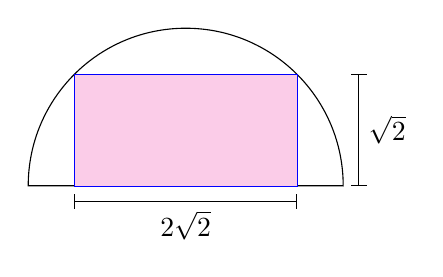
\begin{tikzpicture}[baseline=(current bounding box.north)]
  % Define coordinates
  \def\Radius{2}
  \path
    (-\Radius, 0) coordinate (A)
    -- coordinate (M)
    (\Radius, 0) coordinate (B)
    (M) +(60:\Radius) coordinate (C)
    +(120:\Radius) coordinate (D)
  ;
  % Draw semicircle
  \draw
    (B) arc(0:180:\Radius) -- cycle;
  \filldraw[magenta, fill=magenta!20, ultra thin, draw = blue] (-1.41421356,0) rectangle (1.41421356,1.41421356);
  \draw[|-|](-1.41421356,-0.2)--node[below]{$2\sqrt{2}$}(1.41421356,-0.2);
  \draw[|-|](2.2,0)--node[right]{$\sqrt{2}$}(2.2,1.41421356);
\end{tikzpicture}
\end{center}
Una forma de saber que es correcto el resultado es verificar que el área del rectángulo es menor que el área del semicírculo. Denotando como $A_r$ al área del rectángulo y como $A_{sc}$ al área del semicírculo, se tiene
\begin{align*}
A_r &= \left(2\sqrt{2}\right)\left(\sqrt{2}\right) = 4,\\
A_{sc} &= \dfrac{4\pi}{2} = 2\pi,
\end{align*}
es claro que $A_r < A_{sc}$ por lo que comprobamos que es correcto nuestro resultado.
\end{solution}
 \vspace{0.15in}
%%%%%%%%%%%%%%%%%%%%%%%%%%%%%%%%%%%%%
%           QUESTION                %
%%%%%%%%%%%%%%%%%%%%%%%%%%%%%%%%%%%%%
\question Dada la función $f(x) = \left(x^3 - 3x\right)^2$ determine:
    \begin{parts}
        \part Intervalos donde la función es creciente y decreciente.
    \end{parts}
%%%%%%%%%%%%%%%%%%%%%%%%%%%%%%%%%%%%%%
%             ANSWER                 %
%%%%%%%%%%%%%%%%%%%%%%%%%%%%%%%%%%%%%%
\begin{solution}
Lo que se hará es encontrar los puntos críticos, posteriormente se utilizará el criterio de la segunda derivada para definir cuáles son \textcolor{cyan}{máximos} y cuáles \textcolor{orange}{mínimos} para posteriormente definir los intervalos de crecimiento y decrecimiento.
\begin{enumerate}
    \item Derivar $f(x)$, se tiene
        \begin{align*}
        f'(x) = 2\left(x^3 - 3x\right)\left(3x^2 - 3\right) = 6x\left(x^2 - 3\right)\left(x^2 - 1\right) = 6x^5 - 24x^3 + 18x
        \end{align*}
    \item Para encontrar los puntos críticos se hace $f'(x) = 0$, entonces
        \begin{align*}
        6x\left(x^2 - 3\right)\left(x^2 - 1\right) = 0
        \end{align*}
        de aquí se deduce lo siguiente
        \begin{multicols}{3}
            \begin{itemize}
                \item $x=0$,
                \item $x^2 - 3 = 0 \Rightarrow x = \pm\sqrt{3}$,
                \item $x^2 - 1 = 0 \Rightarrow x = \pm 1$
            \end{itemize}\vspace*{1cm}
        \begin{center}
        \vspace*{\fill}
            $\overrightarrow{entonces}$
        \vspace*{\fill}
        \vspace*{1.29cm}
        \end{center}
            \begin{itemize}
                \item $x_1 = -\sqrt{3}$,
                \item $x_2 = -1$,
                \item $x_3 = 0$,
                \item $x_4 = 1$,
                \item $x_5 = \sqrt{3}$
            \end{itemize}
        \end{multicols}
    \item Se encuentra la segunda derivada de $f(x)$, esto es
        \begin{align*}
        f''(x) = 30x^4 - 72x^2 + 18
        \end{align*}
    \item Definir si son \textcolor{cyan}{máximos} o \textcolor{orange}{mínimos}, esto es haciendo $f''(x_i)$ con $i = 1,\ldots,5$ y analizando su signo.
        \begin{itemize}
            \item $f''(x_1) = 30\left(-\sqrt{3}\right)^4 - 72\left(-\sqrt{3}\right)^2 + 18 = 270 - 216 + 18 = 72 > 0\Rightarrow$ \textcolor{orange}{$x_1$, mínimo},
            \item $f''(x_2) = 30\left(-1\right)^4 - 72\left(-1\right)^2 + 18 = 30 -72 + 18 = -24 < 0\Rightarrow$ \textcolor{cyan}{$x_2$, máximo},
            \item $f''(x_3) = 30\left(0\right)^4 - 72\left(0\right)^2 + 18 = 0 - 0 + 18 = 18 > 0\Rightarrow$ \textcolor{orange}{$x_3$, mínimo},
            \item $f''(x_4) = 30\left(1\right)^4 - 72\left(1\right)^2 + 18 = 30 -72 + 18 = -24 < 0\Rightarrow$ \textcolor{cyan}{$x_4$, máximo},
            \item $f''(x_5) = 30\left(\sqrt{3}\right)^4 - 72\left(\sqrt{3}\right)^2 + 18 = 270 - 216 + 18 = 72 > 0\Rightarrow$ \textcolor{orange}{$x_5$, mínimo}
        \end{itemize}
    \item Se definen los siguientes intervalos y se declara si son crecientes o decrecientes
        \begin{center}
        \begin{tabular}{|c|c|c|c|c|c|}
        \hline
        $\left(-\infty,-\sqrt{3}\right)$ & $\left(-\sqrt{3},-1\right)$ & $\left(-1,0\right)$ & $\left(0,1\right)$ & $\left(1,\sqrt{3}\right)$ & $\left(\sqrt{3},\infty\right)$ \\
        \hline
        \textcolor{red}{decreciente} & \textcolor{blue}{creciente} & \textcolor{red}{decreciente} & \textcolor{blue}{creciente} & \textcolor{red}{decreciente} & \textcolor{blue}{creciente}\\
        \hline
        \end{tabular}
        \captionof{table}{Intervalos de crecimiento y decrecimiento}
        \label{tabla1}
        \end{center}
\end{enumerate}
\begin{center}
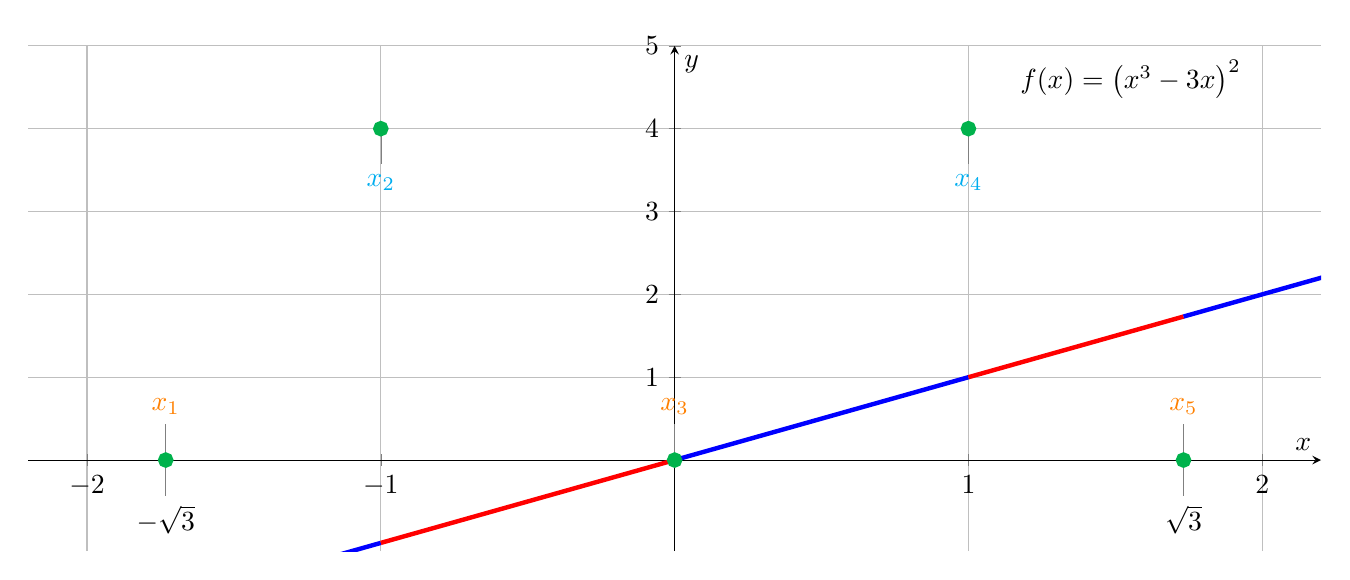
\begin{tikzpicture}
\begin{axis}[
        axis y line=center,
        axis x line=middle,
        % axis on top=true,
        xlabel={$x$},
        ylabel={$y$},
        xmin=-2.2,
        xmax=2.2,
        ymin=-1.1,
        ymax=5,
        height=8.0cm,
        width=18.0cm,
        grid,
        xtick={-2,...,2},
        ytick={0,...,5},
    ]
    \addplot [domain=-3:-1.732051, samples=300, ultra thick, red] {\F(x)};
    \addplot [domain=-1.732051:-1, samples=300, ultra thick, blue] {\F(x)};
    \addplot [domain=-1:0, samples=300, ultra thick, red] {\F(x)};
    \addplot [domain=0:1, samples=300, ultra thick, blue] {\F(x)};
    \addplot [domain=1:1.732051, samples=300, ultra thick, red] {\F(x)};
    \addplot [domain=1.732051:3, samples=300, ultra thick, blue] {\F(x)};
    \node [left, black] at (axis cs: 1.96,4.6) {$f(x) = \left(x^3-3x\right)^2$};
    % \addplot+[only marks, mark = *, blue] coordinates {(-1.732051,0) (-1,4) (0,0) (1,4) (1.732051,0)};
    % \node [coordinate,pin=below:{red mark}]
    %     at (axis cs:0,0) {};
        \addplot[only marks,blue!30!green,ultra thick] coordinates{
        (-1.732051,0)
        (-1,4)
        (0,0)
        (1,4)
        (1.732051,0)
        };
    \node [coordinate,pin=above:{\textcolor{orange}{$x_1$}}] at (axis cs:-1.732051,0) {};
    \node [coordinate,pin=below:{$-\sqrt{3}$}] at (axis cs:-1.732051,0) {};
    \node [coordinate,pin=below:{\textcolor{cyan}{$x_2$}}] at (axis cs:-1,4) {};
    \node [coordinate,pin=above:{\textcolor{orange}{$x_3$}}] at (axis cs:0,0) {};
    \node [coordinate,pin=below:{$\sqrt{3}$}] at (axis cs:1.732051,0) {};
    \node [coordinate,pin=below:{\textcolor{cyan}{$x_4$}}] at (axis cs:1,4) {};
    \node [coordinate,pin=above:{\textcolor{orange}{$x_5$}}] at (axis cs:1.732051,0) {};
\end{axis}
\end{tikzpicture}
\end{center}
\end{solution}
 \newpage
%%%%%%%%%%%%%%%%%%%%%%%%%%%%%%%%%%%%%
%           QUESTION                %
%%%%%%%%%%%%%%%%%%%%%%%%%%%%%%%%%%%%%
\question La concentración de un medicamento en la sangre de un paciente $t$ horas después de una inyección disminuye a una tasa de $C'(t) = \dfrac{-0.33t}{\sqrt{0.02t^2 + 10}}\ mg/cm^3$ por hora. ¿En cuánto cambia la concentración en las primeras 4 horas después de la inyección?
%%%%%%%%%%%%%%%%%%%%%%%%%%%%%%%%%%%%%%
%             ANSWER                 %
%%%%%%%%%%%%%%%%%%%%%%%%%%%%%%%%%%%%%%
\begin{solution}
Nos piden el cambio de la concentración en las primeras 4 horas después de la inyección, es decir, que quieren saber cuánto disminuyo en el intervalo $0\leq t \leq 4$, por lo que lo primero que debemos de encontrar será la concentración, para ello se procederá a integrar la función $C'(t)$ y se tiene
\begin{align*}
\int_0^4 C'(t) dt = \int_0^4 \dfrac{-0.33t}{\sqrt{0.02t^2 + 10}}dt
\end{align*}
se sigue lo siguiente
\begin{multicols}{2}
\begin{align*}
-0.33 \int_0^4 \dfrac{t}{\sqrt{0.02t^2 + 10}}dt
\end{align*}
se resuelve por cambio de variable\\
\begin{align*}
u &= 0.02t^2 + 10\\
\dv{u}{x} &= 2(0.02t)dt = 0.04t dt\Rightarrow \dfrac{1}{0.04} du = t dt
\end{align*}
\end{multicols}
sustituyendo lo anterior se tiene
\begin{align*}
-0.33 \int_0^4 \dfrac{\dfrac{1}{0.04} du}{\sqrt{u}} &= \dfrac{-0.33}{0.04}\int_0^4\dfrac{du}{\sqrt{u}} = \dfrac{-0.33}{0.04}\int_0^4u^{-1/2}du = \dfrac{-0.33}{0.04}\left[\dfrac{u^{-1/2 + 1}}{\dfrac{-1}{2} + 1}\right]_0^4 = \dfrac{-0.33}{0.04}\left[\dfrac{u^{1/2}}{\dfrac{1}{2}}\right]_0^4 \\
&= \dfrac{(2)(-0.33)}{0.04}\left[u^{1/2}\right]_0^4 = \dfrac{33}{2}\left[u^{1/2}\right]_0^4
\end{align*}
sustituyendo $u = 0.02t^2 + 10$ se tiene
\begin{align*}
&= \dfrac{33}{2}\left[\left(0.02t^2 + 10\right)^{1/2}\right]_0^4 = \dfrac{33}{2}\left[\sqrt{0.02t^2 + 10}\right]_0^4 = \dfrac{33}{2}\left[\sqrt{0.02(4)^2 + 10} - \sqrt{0.02(0)^2 + 10}\right] \\
&= \dfrac{33}{2}\left[\sqrt{10.32} - \sqrt{10}\right] \approx -0.8283\ mg/cm^3
\end{align*}
finalmente decimos que la concentración ha cambiado en $-0.8283\ mg/cm^3$ en las primeras 4 horas.
\end{solution}
 \vspace{0.15in}
 %%%%%%%%%%%%%%%%%%%%%%%%%%%%%%%%%%%%%
%           QUESTION                %
%%%%%%%%%%%%%%%%%%%%%%%%%%%%%%%%%%%%%
\question Evalua las siguientes integrales
\begin{align*}
a)\quad\int_{0}^4 \dfrac{xdx}{\sqrt{x^2 + 9}}\qquad\qquad\qquad\qquad\qquad\qquad b)\quad\int x\ln{(x+1)}dx
\end{align*}
 \vspace{0.15in}
%%%%%%%%%%%%%%%%%%%%%%%%%%%%%%%%%%%%%%
%             ANSWER                 %
%%%%%%%%%%%%%%%%%%%%%%%%%%%%%%%%%%%%%%
 \begin{solution}
 \begin{itemize}
 \item[a)] Para la resolución de esta problema se utilizará el método de cambio de variable, entonces se plantea
\begin{multicols}{2}
 \begin{align*}
 u &= x^2 + 9\\
 du &= 2xdx \Rightarrow \dfrac{du}{2} = xdx
 \end{align*}
 entonces se hace el cambio de variable
 \begin{align*}
 \int_0^4 \dfrac{\dfrac{1}{2}du}{\sqrt{u}} = \dfrac{1}{2}\int_0^4 u^{-1/2} du
 \end{align*}
 resolviendo la integral con la formula $\int_a^b u^n du = \left.\dfrac{u^{n+1}}{n+1}\right|_a^b$, entonces
 \begin{align*}
 &\dfrac{1}{2}\left[\dfrac{u^{-1/2+1}}{-\dfrac{1}{2}+1}\right]_0^4 = \cancel{\dfrac{1}{2}}\left[\dfrac{u^{1/2}}{\cancel{\dfrac{1}{2}}}\right]_0^4 = \left[u^1/2\right]_0^4 = \left[x^2 + 9\right]_0^4\\
 &= \sqrt{4^2 + 9} - \sqrt{9} = \sqrt{25} - 3 = 5-3 = 2
 \end{align*}
\end{multicols}
finalmente
\begin{align*}
\int_{0}^4 \dfrac{xdx}{\sqrt{x^2 + 9}} = 2
\end{align*}
\item[b)] Este problema se resuelve por el método de resolución de integración por partes, entonces
\begin{multicols}{2}
se selecciona
\begin{align*}
u = \ln{(x+1)}\qquad\qquad dv = xdx\\
du = \dfrac{dx}{x+1}\qquad\qquad v = \dfrac{1}{2}x^2
\end{align*}
aplicando $uv - \int vdu$ se tiene
\begin{align}
\dfrac{1}{2}x^2\ln{(x+1)} - \dfrac{1}{2}\int \dfrac{x^2}{x+1} dx
\end{align}
\end{multicols}
esta última integral se resuelve por el método de cambio de variable, se hace el cambio $w = x+1\Rightarrow\left(w-1\right)^2 = x^2$, y $dw = dx$, resolviendo esta última integral se tiene
\begin{align*}
\int \dfrac{x^2}{x+1} dx = \int \dfrac{\left(w-1\right)^2}{w} dw = \int\dfrac{w^2 - 2w + 1}{w} dw = \int wdw - 2\int dw + \int \dfrac{1}{w} dw
\end{align*}
que tiene como respuesta es
\begin{align*}
\int \dfrac{x^2}{x+1} dx = \dfrac{w^2}{2} - 2w + \ln{(w)}\ \Rightarrow\ \dfrac{1}{2}\left(x+1\right)^2 - 2\left(x+1\right) + \ln{(x+1)} = \dfrac{x^2 - 2x - 3}{2} + \ln{(x+1)}
\end{align*}
finalmente la respuesta es
\begin{align}
\int x\ln{(x+1)}dx = \dfrac{1}{2}x^2\ln{(x+1)} - \dfrac{1}{4}\left(x^2 - 2x - 3\right) - \dfrac{1}{4}\ln{(x+1)} + C
\end{align}
 \end{itemize}
 \end{solution}
 %%%%%%%%%%%%%%%%%%%%%%%%%%%%%%%%%%%%%
%           QUESTION                %
%%%%%%%%%%%%%%%%%%%%%%%%%%%%%%%%%%%%%
\question Determina el área de la región del plano cartesiano limitada por: La parábola $x^2 - 6x + y = 0$ y la recta $y - x = 0$.
\end{questions}
\vspace{0.15in}
 %%%%%%%%%%%%%%%%%%%%%%%%%%%%%%%%%%%%%
%             ANSWER                 %
%%%%%%%%%%%%%%%%%%%%%%%%%%%%%%%%%%%%%%
\begin{solution}
Primero se graficarán las funciones y se determinará el área entre las curvas con la letra $A$.
\begin{center}
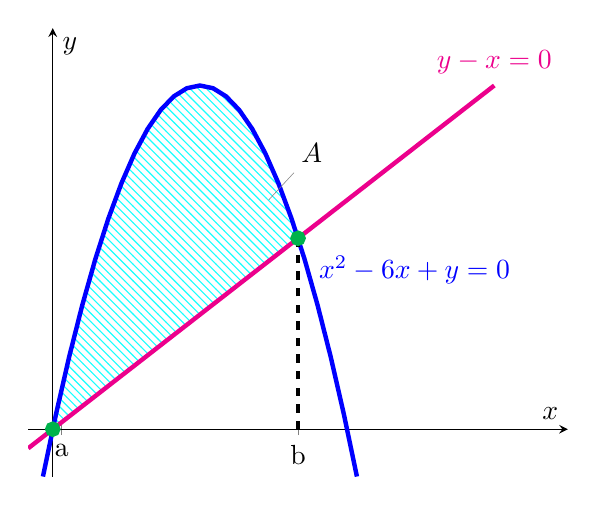
\begin{tikzpicture}
\begin{axis}[axis lines=middle,
            xlabel=$x$,
            ylabel=$y$,
            ymax = 10.5,
            xmax=10.5,
            % enlargelimits,
            ytick=\empty,
            xtick={0.18,5},
            xticklabels={a,b}
            ],
\addplot[name path=F,blue,domain={-.2:6.2}, ultra thick] {-x^2+6*x} node[pos=.75, right]{$x^2 - 6x + y = 0$};
\addplot[name path=G,magenta,domain={-.5:9}, ultra thick] {x}node[pos=1, above]{$y-x=0$};
\addplot[pattern=north west lines, pattern color=cyan!90]fill between[of=F and G, soft clip={domain=0:5}];
\node[coordinate,pin=50:{$A$}] at (axis cs:4.4,6){};
\addplot[only marks,blue!30!green,ultra thick] coordinates{
        (5,5)
        (0,0)
        };
\addplot[dashed, black, ultra thick]coordinates{(5,0) (5,5)};
\end{axis}
% \draw [dashed] (5,0) -- (5,5);
\end{tikzpicture}
\end{center}
posteriormente se usará la formula para calcular el área $A = \int_a^b\Big(g(x) - f(x) \Big) dx$, siendo $a=0$ y $b=5$, además de que se tiene \textcolor{magenta}{$f(x) = x$} y \textcolor{blue}{$g(x) = -x^2+6x$}, por lo que sustituyendo en la formula se tiene.
\begin{align*}
A = \int_0^5\Big(-x^2+6x - x \Big) dx = \int_0^5\Big(-x^2+5x\Big) dx = -\int_0^5 x^2 dx + 5\int_0^5 x dx = \left.-\dfrac{1}{3}x^3+\dfrac{5}{2}x^2\right|_0^5
\end{align*}
por lo tanto
\begin{align*}
\left.-\dfrac{1}{3}x^3+\dfrac{5}{2}x^2\right|_0^5 = \left[-\dfrac{1}{3}(5)^3+\dfrac{5}{2}(5)^2\right] - \left[-\dfrac{1}{3}(0)^3+\dfrac{5}{2}(0)^2\right] = -\dfrac{125}{3} + \dfrac{125}{2} = 125\left(\dfrac{-1}{3} + \dfrac{1}{2}\right) = \dfrac{125}{6}
\end{align*}
finalmente el área entre las curvas es $A = \dfrac{125}{6} u^2$.
\end{solution}
\end{document}
